\section{$B$-mesons and track classification}

$B$-mesons are mesons composed of one $b$-quark and another lighter quark.
Relevant for this thesis are the uncharged $B$-mesons
\begin{align*}
    B^0 &= b\bar{d} \, , & \bar{B}^0 &= \bar{b}d \, , & B_s^0 &= b\bar{s} \, , & \bar{B}_s^0 &= \bar{b}s \, .
\end{align*}
    
In a $pp$-collision $B$-mesons are produced in pairs, because of the production of $b\bar{b}$-pairs through the strong interaction. 
The $B$-meson of interest for an analysis is called the signal $B$ and its partner is called the opposite $B$.
The underlying event is therefore often divided into same side tracks and opposite side tracks, depending on the origin of its particle.
Each side can then be further divided into fragmentation tracks and decay tracks. (see \autoref{fig:ft_scheme})
At LHCb, this track classification is often used in flavour tagging algorithms, and it is also used in this thesis.

\begin{figure}
    \centering
    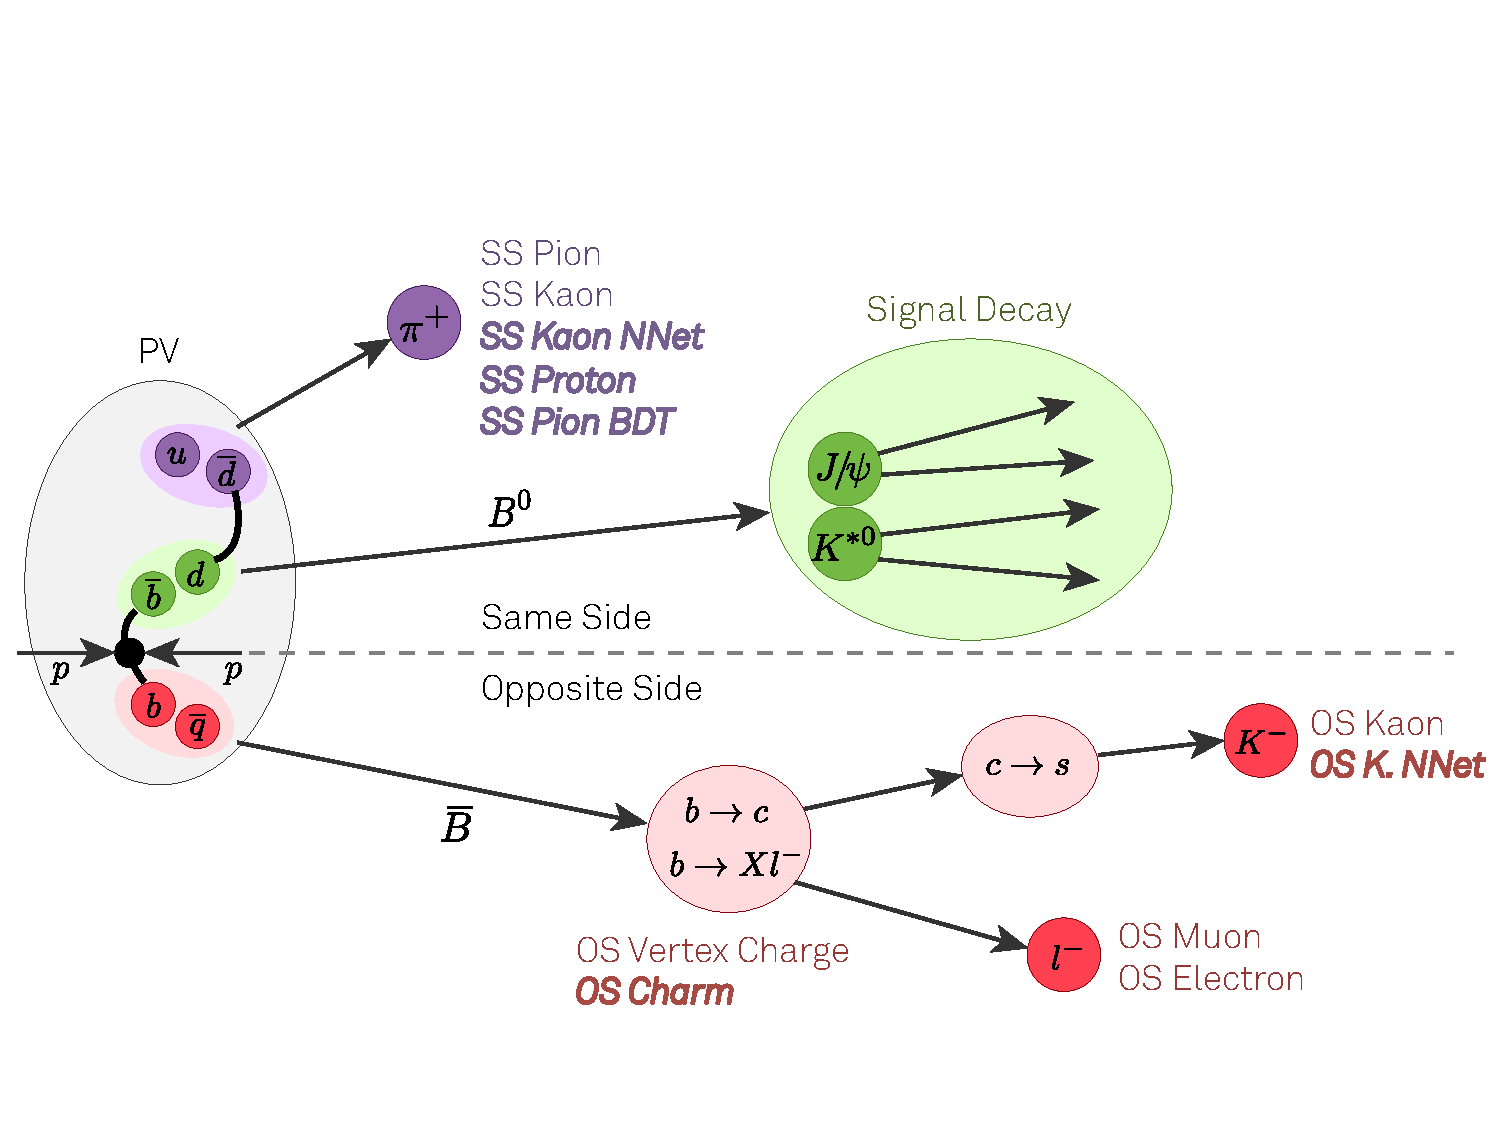
\includegraphics[width=\textwidth]{images/FlavourTaggingScheme.pdf}
    \caption{Track classification used in flavour tagging algorithms. \cite{ft_scheme}}
    \label{fig:ft_scheme}
\end{figure}


%\begin{table}
%    \centering
%    \caption{Listing of $B$-mesons and their quark contents.}
%    \begin{tabular}{c c c c | c c c c}
%        \toprule
%        \multicolumn{4}{c}{uncharged $B$-mesons} & \multicolumn{4}{c}{charged $B$-mesons} \\
%        \midrule
%        $B_d^0$ & $\bar{B}_d^0$ & $B_s^0$ & $\bar{B}_s^0$ & $B_u^-$ & $B_u^+$ & $B_c^-$ & $B_c^+$ \\
%        $b\bar{d}$ & $\bar{b}d$ & $b\bar{s}$ & $\bar{b}s$ & $b\bar{u}$ & $\bar{b}u$ & $b\bar{c}$ & $\bar{b}c$ \\
%        \bottomrule
%    \end{tabular}
%    \label{tab:B_mesons}
%\end{table}

%\begin{table}
%    \centering
%    \caption{Listing of $B$-mesons and their quark contents.}
%    \begin{tabular}{c c | c c}
%        \toprule
%        \multicolumn{2}{c}{uncharged $B$-mesons} & \multicolumn{2}{c}{charged $B$-mesons} \\
%        \midrule
%        $B^0 = b\bar{d}$ & $B_s^0 = b\bar{s}$ & $B^- = b\bar{u}$ & $B_c^- = b\bar{c}$ \\
%        $\bar{B}^0 = \bar{b}d$ & $\bar{B}_s^0 = \bar{b}s$ & $B^+ = \bar{b}u$ & $B_c^+ = \bar{b}c$ \\
%        \bottomrule
%    \end{tabular}
%    \label{tab:B_mesons}
%\end{table}

%\begin{align*}
%    \text{uncharged:} & B_d^0 = b\bar{d}, & \bar{B}_d^0 = \bar{b}d, & B_s^0 = b\bar{s}, & \bar{B}_s^0 = \bar{b}s \\
%    \text{charged:} & B_u^- = b\bar{u} & B_u^+ = \bar{b}u & B_c^- = b\bar{c} & B_c^+ = \bar{b}c
%\end{align*}



%The decay channels used in this thesis are
%\begin{align*}
%    B_d^0/\bar{B}_d^0 &\rightarrow J/\psi + K*^0 \, , \\
%    B_s^0/\bar{B}_s^0 &\rightarrow D_s^- + \pi^+ \, \text{and} \\
%    B_d^0/\bar{B}_d^0/B_s^0/\bar{B}_s^0 &\rightarrow J/\psi + K_S^0 \, .
%\end{align*}